% L04_mini5.tex -- Fintech Security and Regulation
% 5-Slide Teaser Arc: WHY > WHAT > HOW > WHERE > SO WHAT
% Self-contained (no \input{} commands, no \includegraphics)
% Compile: pdflatex L04_mini5.tex (twice for overlays)
% ============================================================

\documentclass[aspectratio=169, 11pt]{beamer}
\usetheme{Madrid}
\usecolortheme{whale}
\usepackage{tikz,pgfplots,booktabs,multicol,amsmath}
\usetikzlibrary{arrows.meta,positioning,shapes.geometric,calc,decorations.pathmorphing}
\pgfplotsset{compat=1.18}

% ---- Colour palette ----------------------------------------
\definecolor{mlpurple}{HTML}{9467BD}
\definecolor{mlblue}{HTML}{1F77B4}
\definecolor{mlred}{HTML}{D62728}
\definecolor{mlorange}{HTML}{FF7F0E}
\definecolor{mlgreen}{HTML}{2CA02C}
\definecolor{mlgray}{HTML}{7F7F7F}
\definecolor{mlteal}{HTML}{0D7377}
\definecolor{mlcyan}{HTML}{14BDEB}

% ---- Beamer theme colours ----------------------------------
\setbeamercolor{structure}{fg=mlteal}
\setbeamercolor{palette primary}{bg=mlteal,fg=white}
\setbeamercolor{palette secondary}{bg=mlteal!80,fg=white}
\setbeamercolor{palette tertiary}{bg=mlteal!60,fg=white}
\setbeamercolor{frametitle}{bg=mlteal!10,fg=mlteal}
\setbeamercolor{title}{fg=white}
\setbeamercolor{subtitle}{fg=mlcyan!80}
\setbeamercolor{block title}{bg=mlteal,fg=white}
\setbeamercolor{block body}{bg=mlteal!8,fg=black}
\setbeamercolor{block title alerted}{bg=mlred!80,fg=white}
\setbeamercolor{block body alerted}{bg=mlred!8,fg=black}

% ---- Bottom-note command -----------------------------------
\newcommand{\bottomnote}[1]{%
  \vfill
  \begin{beamercolorbox}[wd=\textwidth,ht=2ex,dp=1ex]{palette primary}%
    \tiny\hspace{1em}#1%
  \end{beamercolorbox}}

% ---- Metadata ----------------------------------------------
\title{Fintech Security and Regulation}
\subtitle{5-Slide Teaser}
\author{Joerg Osterrieder}
\institute{University of Zurich}
\date{Spring 2026}
\setbeamertemplate{navigation symbols}{}

% ============================================================
\begin{document}
% ============================================================

% -----------------------------------------------------------
%  TITLE FRAME (not counted in the 5)
% -----------------------------------------------------------
\begin{frame}
  \titlepage
  \bottomnote{Financial Technology (FinTech) -- MSc Course | University of Zurich | Spring 2026}
\end{frame}

% ===========================================================
%  SLIDE 1 of 5  --  WHY
%  Visual: TikZ comic -- balance scale: Innovation vs Regulation
% ===========================================================
\begin{frame}{Why Regulate Fintech? The Innovation--Regulation Balancing Act}

\begin{center}
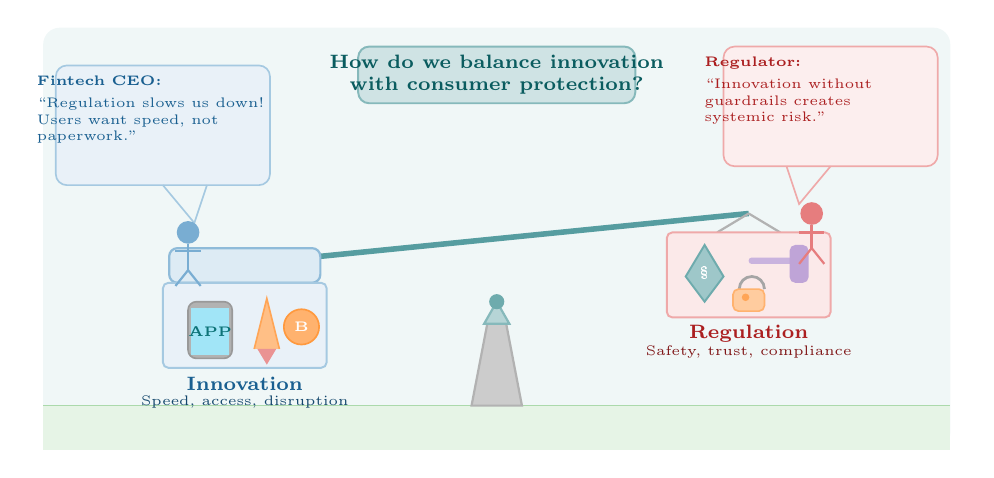
\begin{tikzpicture}[scale=0.80, every node/.style={font=\small}]

  % ---- Background ----
  \fill[mlteal!6, rounded corners=6pt] (-7.2,-3.2) rectangle (7.2,3.5);

  % ---- Ground ----
  \fill[mlgreen!12] (-7.2,-3.2) rectangle (7.2,-2.5);
  \draw[mlgreen!40, line width=0.5pt] (-7.2,-2.5) -- (7.2,-2.5);

  % ============ BALANCE SCALE (centre) ============

  % Fulcrum / pedestal
  \fill[mlgray!40, draw=mlgray!60, line width=0.8pt]
    (-0.4,-2.5) -- (0.4,-2.5) -- (0.15,-1.2) -- (-0.15,-1.2) -- cycle;
  \fill[mlteal!30, draw=mlteal!50, line width=0.8pt]
    (-0.2,-1.2) -- (0.2,-1.2) -- (0.0,-0.85) -- cycle;

  % Beam (tilted slightly: innovation side heavier / lower)
  \draw[mlteal!70, line width=2.0pt, rounded corners=1pt]
    (-4.0,-0.25) -- (4.0,0.55);
  \fill[mlteal!60] (0.0,-0.85) circle (0.12);

  % ---- LEFT PAN: Innovation (heavier, lower) ----
  % Pan chains
  \draw[mlgray!60, line width=0.8pt] (-4.0,-0.25) -- (-4.5,-0.55);
  \draw[mlgray!60, line width=0.8pt] (-4.0,-0.25) -- (-3.5,-0.55);
  % Pan
  \fill[mlblue!15, draw=mlblue!50, line width=0.8pt, rounded corners=3pt]
    (-5.2,-0.55) rectangle (-2.8,0.0);
  \draw[mlblue!40, line width=0.6pt] (-5.2,-0.55) -- (-5.2,-1.9);
  \draw[mlblue!40, line width=0.6pt] (-2.8,-0.55) -- (-2.8,-1.9);
  \fill[mlblue!10, draw=mlblue!40, line width=0.7pt, rounded corners=2pt]
    (-5.3,-1.9) rectangle (-2.7,-0.55);

  % Innovation items on left pan
  % Smartphone
  \fill[mlgray!60, draw=mlgray!80, line width=0.6pt, rounded corners=3pt]
    (-4.9,-1.75) rectangle (-4.2,-0.85);
  \fill[mlcyan!40] (-4.85,-1.70) rectangle (-4.25,-0.95);
  \node[font=\tiny\bfseries, text=mlteal] at (-4.55,-1.32) {APP};
  % Rocket
  \fill[mlorange!50] (-3.85,-1.6) -- (-3.65,-0.8) -- (-3.45,-1.6) -- cycle;
  \fill[mlred!50] (-3.80,-1.6) -- (-3.65,-1.85) -- (-3.50,-1.6) -- cycle;
  \draw[mlorange!70, line width=0.6pt] (-3.85,-1.6) -- (-3.65,-0.8) -- (-3.45,-1.6);
  % Bitcoin symbol
  \fill[mlorange!60, draw=mlorange!80, line width=0.6pt]
    (-3.1,-1.25) circle (0.28);
  \node[font=\tiny\bfseries, text=white] at (-3.1,-1.25) {B};

  \node[font=\scriptsize\bfseries, text=mlblue!80!black] at (-4.0,-2.15)
    {Innovation};
  \node[font=\tiny, text=mlblue!60!black, align=center] at (-4.0,-2.45)
    {Speed, access, disruption};

  % ---- RIGHT PAN: Regulation (lighter, higher) ----
  % Pan chains
  \draw[mlgray!60, line width=0.8pt] (4.0,0.55) -- (3.5,0.25);
  \draw[mlgray!60, line width=0.8pt] (4.0,0.55) -- (4.5,0.25);
  % Pan
  \fill[mlred!10, draw=mlred!40, line width=0.7pt, rounded corners=2pt]
    (2.7,0.25) rectangle (5.3,-1.1);

  % Regulation items on right pan
  % Shield
  \fill[mlteal!40, draw=mlteal!60, line width=0.7pt]
    (3.3,0.05) -- (3.0,-0.45) -- (3.3,-0.85) -- (3.6,-0.45) -- cycle;
  \node[font=\tiny\bfseries, text=white] at (3.3,-0.40) {\S};
  % Gavel
  \fill[mlpurple!50, rounded corners=1pt] (4.0,-0.25) rectangle (4.8,-0.15);
  \fill[mlpurple!60, rounded corners=2pt] (4.65,-0.55) rectangle (4.95,0.05);
  % Lock
  \draw[mlgray!70, line width=1.0pt] (4.25,-0.65) arc (0:180:0.2);
  \fill[mlorange!40, draw=mlorange!60, line width=0.6pt, rounded corners=2pt]
    (3.75,-0.65) rectangle (4.25,-1.0);
  \fill[mlorange!70] (3.95,-0.78) circle (0.06);

  \node[font=\scriptsize\bfseries, text=mlred!80!black] at (4.0,-1.35)
    {Regulation};
  \node[font=\tiny, text=mlred!60!black, align=center] at (4.0,-1.65)
    {Safety, trust, compliance};

  % ============ SPEECH BUBBLES ============

  % Left bubble: Innovator
  \fill[mlblue!10, draw=mlblue!40, line width=0.6pt, rounded corners=4pt]
    (-7.0,1.0) rectangle (-3.6,2.9);
  \draw[mlblue!40, line width=0.6pt]
    (-5.3,1.0) -- (-4.8,0.4) -- (-4.6,1.0);
  \node[font=\tiny, text=mlblue!80!black, align=left, text width=3.2cm]
    at (-5.3,2.2)
    {\textbf{Fintech CEO:}\\[2pt]``Regulation slows us down!\\
     Users want speed, not\\paperwork.''};

  % Stick figure (innovator)
  \fill[mlblue!60] (-4.9,0.25) circle (0.18);
  \draw[mlblue!60, line width=1.0pt] (-4.9,0.07) -- (-4.9,-0.35);
  \draw[mlblue!60, line width=0.8pt] (-5.1,-0.05) -- (-4.7,-0.05);
  \draw[mlblue!60, line width=0.8pt] (-4.9,-0.35) -- (-5.1,-0.6);
  \draw[mlblue!60, line width=0.8pt] (-4.9,-0.35) -- (-4.7,-0.6);

  % Right bubble: Regulator
  \fill[mlred!8, draw=mlred!40, line width=0.6pt, rounded corners=4pt]
    (3.6,1.3) rectangle (7.0,3.2);
  \draw[mlred!40, line width=0.6pt]
    (4.6,1.3) -- (4.8,0.7) -- (5.3,1.3);
  \node[font=\tiny, text=mlred!80!black, align=left, text width=3.2cm]
    at (5.3,2.5)
    {\textbf{Regulator:}\\[2pt]``Innovation without\\guardrails creates\\systemic risk.''};

  % Stick figure (regulator)
  \fill[mlred!60] (5.0,0.55) circle (0.18);
  \draw[mlred!60, line width=1.0pt] (5.0,0.37) -- (5.0,-0.0);
  \draw[mlred!60, line width=0.8pt] (4.8,0.25) -- (5.2,0.25);
  \draw[mlred!60, line width=0.8pt] (5.0,0.0) -- (4.8,-0.25);
  \draw[mlred!60, line width=0.8pt] (5.0,0.0) -- (5.2,-0.25);

  % ---- Central question ----
  \fill[mlteal!20, rounded corners=4pt, draw=mlteal!50, line width=0.7pt]
    (-2.2,2.3) rectangle (2.2,3.2);
  \node[font=\scriptsize\bfseries, text=mlteal!80!black, align=center]
    at (0.0,2.75)
    {How do we balance innovation\\with consumer protection?};

\end{tikzpicture}
\end{center}

\bottomnote{Slide 1/5 --- WHY | Financial Technology -- MSc | University of Zurich | Spring 2026}
\end{frame}

% ===========================================================
%  SLIDE 2 of 5  --  WHAT
%  Visual: Table comparing regulatory approaches across jurisdictions
% ===========================================================
\begin{frame}[shrink=5]{What Are the Regulatory Approaches? A Global Comparison}

\vspace{-0.1em}
\begin{center}
\textcolor{mlteal}{\textbf{\small Comparing Fintech Regulatory Frameworks Across Major Jurisdictions}}
\vspace{0.5em}

\scriptsize
\setlength{\tabcolsep}{4pt}
\renewcommand{\arraystretch}{1.30}
\begin{tabular}{@{}lp{2.4cm}p{2.2cm}p{2.2cm}p{2.2cm}p{2.2cm}@{}}
  \toprule
  \textbf{Jurisdiction} & \textbf{Approach} & \textbf{Crypto / DeFi} & \textbf{Sandbox?} & \textbf{Key Legislation} & \textbf{Strength / Weakness} \\
  \midrule
  \textbf{United States} &
    Patchwork; multi-agency (SEC, CFTC, OCC, FinCEN) &
    \textcolor{mlred}{Fragmented}: SEC vs CFTC turf battles &
    \textcolor{mlorange!80!black}{Limited} (state-level) &
    BSA/AML, state MTLs, proposed FIT21 &
    \textcolor{mlgreen!70!black}{Deep markets} / \textcolor{mlred}{regulatory uncertainty} \\[3pt]

  \textbf{European Union} &
    Harmonised; single-market rules &
    \textcolor{mlgreen!70!black}{MiCA} (2024): unified crypto framework &
    \textcolor{mlgreen!70!black}{Yes} (national level) &
    MiCA, PSD2/PSD3, DORA, GDPR &
    \textcolor{mlgreen!70!black}{Legal clarity} / \textcolor{mlred}{compliance burden} \\[3pt]

  \textbf{United Kingdom} &
    Activity-based; FCA-led &
    Evolving; crypto promotion rules &
    \textcolor{mlgreen!70!black}{Pioneer} (FCA sandbox 2016) &
    FSMA, PSRs, crypto regime TBD &
    \textcolor{mlgreen!70!black}{Sandbox model} / \textcolor{mlorange!80!black}{post-Brexit divergence} \\[3pt]

  \textbf{Singapore} &
    Licensing tiers; MAS-led &
    \textcolor{mlgreen!70!black}{PSA}: tiered crypto licensing &
    \textcolor{mlgreen!70!black}{Yes} (MAS sandbox) &
    PSA 2019, licensing tiers (SPI, MPI, DPT) &
    \textcolor{mlgreen!70!black}{Clear tiers} / \textcolor{mlorange!80!black}{small domestic market} \\
  \bottomrule
\end{tabular}
\end{center}

\vspace{0.3em}
\begin{columns}[T]
\begin{column}{0.48\textwidth}
  \begin{block}{No Global Standard}
    \scriptsize
    Regulatory fragmentation creates arbitrage opportunities.
    Firms ``jurisdiction shop'' for the most favourable regime,
    raising concerns about a \textbf{race to the bottom}.
  \end{block}
\end{column}
\begin{column}{0.48\textwidth}
  \begin{alertblock}{\scriptsize The Sandbox Paradigm}
    \scriptsize
    Regulatory sandboxes let firms test innovations under
    \textbf{relaxed rules with guardrails}. Over 70 countries
    now operate some form of sandbox programme.
  \end{alertblock}
\end{column}
\end{columns}

\bottomnote{Slide 2/5 --- WHAT | Financial Technology -- MSc | University of Zurich | Spring 2026}
\end{frame}

% ===========================================================
%  SLIDE 3 of 5  --  HOW
%  Visual: TikZ diagram -- money laundering stages
% ===========================================================
\begin{frame}{How Does Money Laundering Work? The Three Stages}

\begin{center}
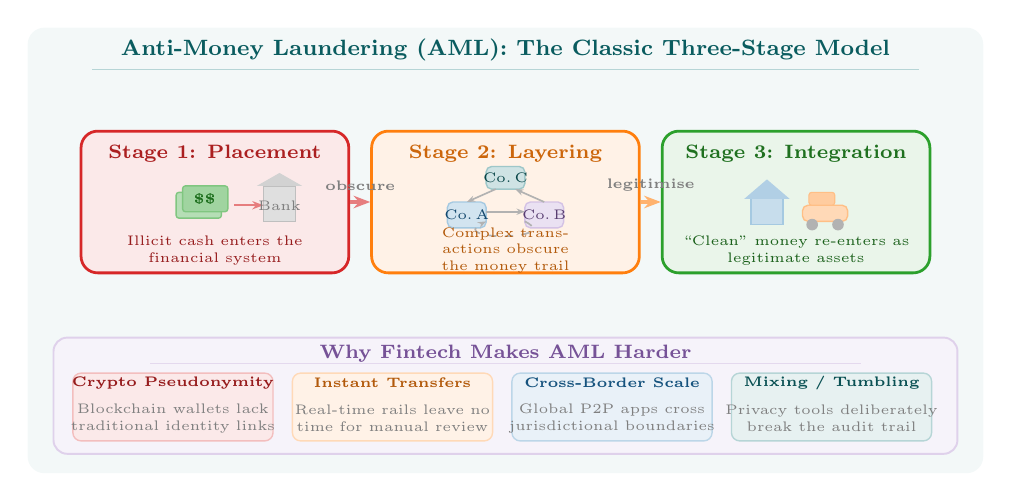
\begin{tikzpicture}[
    scale=0.82,
    stagebox/.style={rectangle, rounded corners=6pt, minimum width=3.4cm,
                minimum height=1.8cm, align=center, font=\scriptsize,
                line width=1.0pt, draw, inner sep=6pt},
    arr/.style={-{Stealth[length=6pt]}, line width=1.4pt},
    every node/.style={font=\small}
  ]

  % ---- Background ----
  \fill[mlteal!5, rounded corners=6pt] (-7.4,-3.4) rectangle (7.4,3.5);

  % ---- Title ----
  \node[font=\footnotesize\bfseries, text=mlteal!80!black] at (0,3.15)
    {Anti-Money Laundering (AML): The Classic Three-Stage Model};
  \draw[mlteal!30, line width=0.4pt] (-6.4,2.85) -- (6.4,2.85);

  % ============ STAGE 1: PLACEMENT (left) ============
  \node[stagebox, fill=mlred!10, draw=mlred]
    (S1) at (-4.5,0.8) {};

  \node[font=\scriptsize\bfseries, text=mlred!80!black] at (-4.5,1.55)
    {Stage 1: Placement};

  % Cash icon: stack of bills
  \fill[mlgreen!35, draw=mlgreen!60, line width=0.5pt, rounded corners=1pt]
    (-5.1,0.55) rectangle (-4.4,0.95);
  \fill[mlgreen!45, draw=mlgreen!60, line width=0.5pt, rounded corners=1pt]
    (-5.0,0.65) rectangle (-4.3,1.05);
  \node[font=\tiny\bfseries, text=mlgreen!70!black] at (-4.65,0.85) {\$\$};
  % Arrow into bank
  \draw[mlred!60, -{Stealth[length=4pt]}, line width=0.8pt]
    (-4.2,0.75) -- (-3.75,0.75);
  % Bank icon (simplified)
  \fill[mlgray!25, draw=mlgray!50, line width=0.5pt]
    (-3.75,0.50) rectangle (-3.25,1.05);
  \fill[mlgray!35] (-3.85,1.05) -- (-3.50,1.25) -- (-3.15,1.05) -- cycle;
  \node[font=\tiny, text=mlgray] at (-3.50,0.75) {Bank};

  \node[font=\tiny, text=mlred!70!black, align=center, text width=3.0cm]
    at (-4.5,0.05)
    {Illicit cash enters the\\financial system};

  % ============ STAGE 2: LAYERING (centre) ============
  \node[stagebox, fill=mlorange!10, draw=mlorange]
    (S2) at (0,0.8) {};

  \node[font=\scriptsize\bfseries, text=mlorange!80!black] at (0,1.55)
    {Stage 2: Layering};

  % Complex web of arrows (shell companies)
  \fill[mlblue!20, draw=mlblue!40, line width=0.5pt, rounded corners=2pt]
    (-0.9,0.4) rectangle (-0.3,0.8);
  \node[font=\tiny, text=mlblue!60!black] at (-0.6,0.6) {Co.\,A};

  \fill[mlpurple!20, draw=mlpurple!40, line width=0.5pt, rounded corners=2pt]
    (0.3,0.4) rectangle (0.9,0.8);
  \node[font=\tiny, text=mlpurple!60!black] at (0.6,0.6) {Co.\,B};

  \fill[mlteal!20, draw=mlteal!40, line width=0.5pt, rounded corners=2pt]
    (-0.3,1.0) rectangle (0.3,1.35);
  \node[font=\tiny, text=mlteal!60!black] at (0.0,1.175) {Co.\,C};

  % Arrows between shell companies
  \draw[mlgray!60, -{Stealth[length=3pt]}, line width=0.6pt]
    (-0.3,0.65) -- (0.3,0.65);
  \draw[mlgray!60, -{Stealth[length=3pt]}, line width=0.6pt]
    (0.6,0.8) -- (0.15,1.0);
  \draw[mlgray!60, -{Stealth[length=3pt]}, line width=0.6pt]
    (-0.15,1.0) -- (-0.6,0.8);
  \draw[mlgray!60, -{Stealth[length=3pt]}, line width=0.6pt, dashed]
    (0.3,0.5) .. controls (0.9,0.2) and (-0.9,0.2) .. (-0.3,0.5);

  \node[font=\tiny, text=mlorange!70!black, align=center, text width=3.0cm]
    at (0,0.05)
    {Complex transactions obscure\\the money trail};

  % ============ STAGE 3: INTEGRATION (right) ============
  \node[stagebox, fill=mlgreen!10, draw=mlgreen]
    (S3) at (4.5,0.8) {};

  \node[font=\scriptsize\bfseries, text=mlgreen!70!black] at (4.5,1.55)
    {Stage 3: Integration};

  % Legitimate assets: house + car icons
  % House
  \fill[mlblue!25, draw=mlblue!40, line width=0.5pt]
    (3.8,0.45) rectangle (4.3,0.85);
  \fill[mlblue!35] (3.7,0.85) -- (4.05,1.15) -- (4.4,0.85) -- cycle;
  % Car (simplified)
  \fill[mlorange!30, draw=mlorange!50, line width=0.5pt, rounded corners=2pt]
    (4.6,0.50) rectangle (5.3,0.75);
  \fill[mlorange!40, draw=mlorange!50, line width=0.4pt, rounded corners=1pt]
    (4.7,0.75) rectangle (5.1,0.95);
  \fill[mlgray!60] (4.75,0.45) circle (0.09);
  \fill[mlgray!60] (5.15,0.45) circle (0.09);

  \node[font=\tiny, text=mlgreen!60!black, align=center, text width=3.0cm]
    at (4.5,0.05)
    {``Clean'' money re-enters as\\legitimate assets};

  % ============ CONNECTING ARROWS ============
  \draw[arr, mlred!60] (S1.east) -- (S2.west)
    node[midway, above, font=\tiny\bfseries, text=mlgray] {obscure};
  \draw[arr, mlorange!60] (S2.east) -- (S3.west)
    node[midway, above, font=\tiny\bfseries, text=mlgray] {legitimise};

  % ============ BOTTOM: FINTECH CHALLENGES ============
  \fill[mlpurple!8, rounded corners=5pt, draw=mlpurple!30, line width=0.7pt]
    (-7.0,-3.1) rectangle (7.0,-1.3);

  \node[font=\scriptsize\bfseries, text=mlpurple!80!black] at (0,-1.55)
    {Why Fintech Makes AML Harder};
  \draw[mlpurple!25, line width=0.3pt] (-5.5,-1.7) -- (5.5,-1.7);

  % Four challenge boxes
  \fill[mlred!10, rounded corners=3pt, draw=mlred!30, line width=0.5pt]
    (-6.7,-2.9) rectangle (-3.6,-1.85);
  \node[font=\tiny\bfseries, text=mlred!70!black] at (-5.15,-2.0)
    {Crypto Pseudonymity};
  \node[font=\tiny, text=mlgray, align=center, text width=2.8cm]
    at (-5.15,-2.55)
    {Blockchain wallets lack\\traditional identity links};

  \fill[mlorange!10, rounded corners=3pt, draw=mlorange!30, line width=0.5pt]
    (-3.3,-2.9) rectangle (-0.2,-1.85);
  \node[font=\tiny\bfseries, text=mlorange!70!black] at (-1.75,-2.0)
    {Instant Transfers};
  \node[font=\tiny, text=mlgray, align=center, text width=2.8cm]
    at (-1.75,-2.55)
    {Real-time rails leave no\\time for manual review};

  \fill[mlblue!10, rounded corners=3pt, draw=mlblue!30, line width=0.5pt]
    (0.1,-2.9) rectangle (3.2,-1.85);
  \node[font=\tiny\bfseries, text=mlblue!70!black] at (1.65,-2.0)
    {Cross-Border Scale};
  \node[font=\tiny, text=mlgray, align=center, text width=2.8cm]
    at (1.65,-2.55)
    {Global P2P apps cross\\jurisdictional boundaries};

  \fill[mlteal!10, rounded corners=3pt, draw=mlteal!30, line width=0.5pt]
    (3.5,-2.9) rectangle (6.6,-1.85);
  \node[font=\tiny\bfseries, text=mlteal!70!black] at (5.05,-2.0)
    {Mixing / Tumbling};
  \node[font=\tiny, text=mlgray, align=center, text width=2.8cm]
    at (5.05,-2.55)
    {Privacy tools deliberately\\break the audit trail};

\end{tikzpicture}
\end{center}

\bottomnote{Slide 3/5 --- HOW | Financial Technology -- MSc | University of Zurich | Spring 2026}
\end{frame}

% ===========================================================
%  SLIDE 4 of 5  --  WHERE
%  Visual: pgfplots bar chart -- compliance costs by firm type
% ===========================================================
\begin{frame}{Where Do Compliance Costs Fall? Burden by Firm Type}

\vspace{-0.4em}
\begin{center}
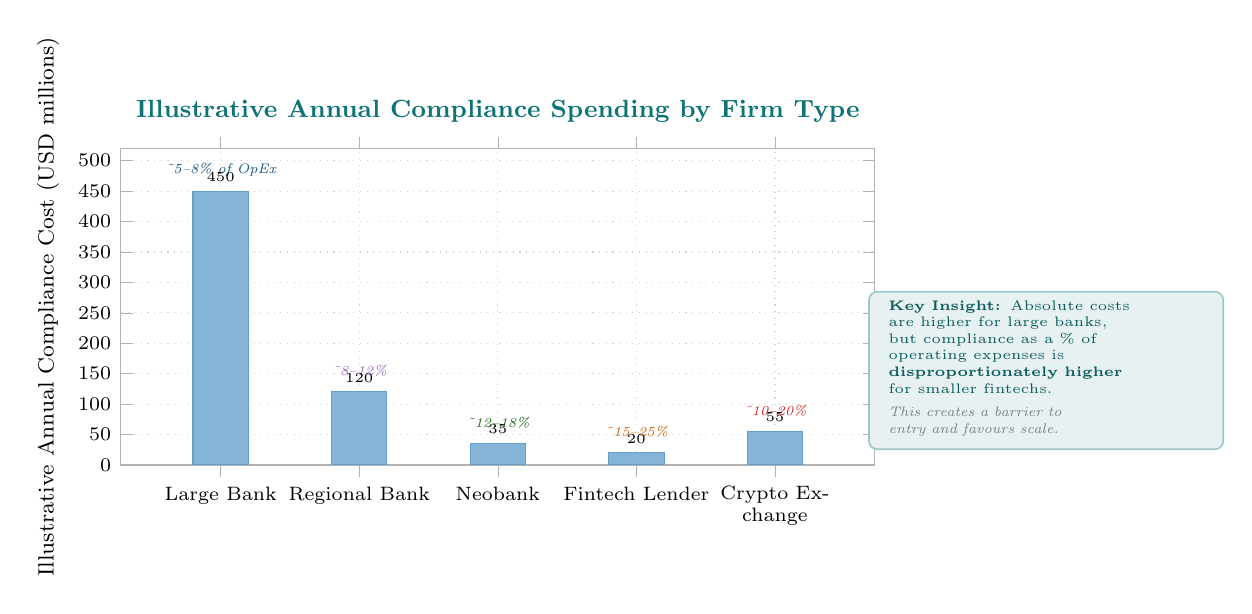
\begin{tikzpicture}
\begin{axis}[
    ybar,
    bar width=20pt,
    width=0.92\textwidth,
    height=5.6cm,
    enlarge x limits=0.18,
    ylabel={\footnotesize Illustrative Annual Compliance Cost (USD millions)},
    ylabel style={font=\scriptsize},
    ymin=0, ymax=520,
    ytick={0,50,100,150,200,250,300,350,400,450,500},
    yticklabel style={font=\scriptsize},
    yticklabel={\pgfmathprintnumber[fixed,precision=0]{\tick}},
    symbolic x coords={Large Bank, Regional Bank, Neobank, Fintech Lender, Crypto Exchange},
    xtick=data,
    xticklabel style={font=\scriptsize, align=center, text width=2.0cm},
    grid=major,
    grid style={dotted, mlgray!35},
    axis line style={mlgray!60},
    tick style={mlgray!60},
    title={\small Illustrative Annual Compliance Spending by Firm Type},
    title style={font=\small\bfseries, color=mlteal},
    nodes near coords,
    nodes near coords style={font=\tiny\bfseries, color=black},
    every node near coord/.append style={/pgf/number format/fixed, /pgf/number format/precision=0}
  ]

  \addplot[fill=mlblue!55, draw=mlblue!70] coordinates {
    (Large Bank,      450)
    (Regional Bank,   120)
    (Neobank,          35)
    (Fintech Lender,   20)
    (Crypto Exchange,  55)
  };

  % Cost-as-%-of-revenue labels
  \node[font=\tiny\itshape, text=mlblue!70!black, align=center]
    at (axis cs:Large Bank, 485)
    {\textasciitilde 5--8\% of OpEx};
  \node[font=\tiny\itshape, text=mlpurple, align=center]
    at (axis cs:Regional Bank, 155)
    {\textasciitilde 8--12\%};
  \node[font=\tiny\itshape, text=mlgreen!70!black, align=center]
    at (axis cs:Neobank, 70)
    {\textasciitilde 12--18\%};
  \node[font=\tiny\itshape, text=mlorange!80!black, align=center]
    at (axis cs:Fintech Lender, 55)
    {\textasciitilde 15--25\%};
  \node[font=\tiny\itshape, text=mlred, align=center]
    at (axis cs:Crypto Exchange, 90)
    {\textasciitilde 10--20\%};

\end{axis}

% Annotation box (bottom right)
\fill[mlteal!10, rounded corners=3pt, draw=mlteal!40, line width=0.6pt]
  (9.5,0.2) rectangle (14.0,2.2);
\node[font=\tiny, text=mlteal!80!black, align=left, text width=4.0cm]
  at (11.75,1.5)
  {\textbf{Key Insight:} Absolute costs\\are higher for large banks,\\but compliance as a \% of\\operating expenses is\\
  \textbf{disproportionately higher}\\for smaller fintechs.};
\node[font=\tiny\itshape, text=mlgray, align=left, text width=4.0cm]
  at (11.75,0.55)
  {This creates a barrier to\\entry and favours scale.};

\end{tikzpicture}
\end{center}

\vspace{-0.6em}
{\tiny\textcolor{mlgray}{\textit{All figures are purely illustrative for teaching purposes. Actual costs vary by jurisdiction, firm maturity, product scope, and regulatory regime.}}}

\bottomnote{Slide 4/5 --- WHERE | Financial Technology -- MSc | University of Zurich | Spring 2026}
\end{frame}

% ===========================================================
%  SLIDE 5 of 5  --  SO WHAT
%  Visual: Evaluation framework for regulatory regimes + RegTech
% ===========================================================
\begin{frame}{So What? Evaluating Regulatory Regimes and the RegTech Promise}

\begin{center}
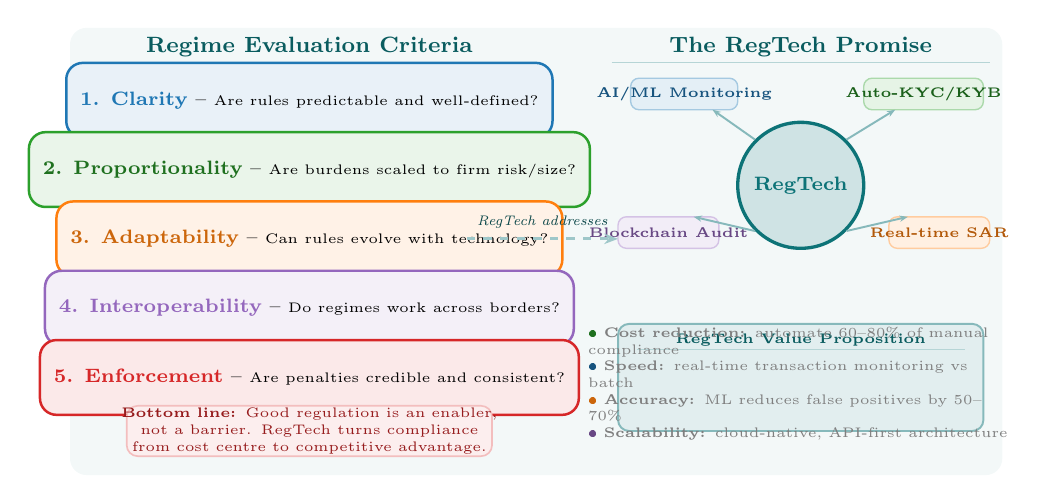
\begin{tikzpicture}[
    scale=0.80,
    qbox/.style={rectangle, rounded corners=6pt, minimum width=4.8cm,
                 minimum height=0.95cm, align=left, font=\scriptsize,
                 line width=0.9pt, draw, inner sep=5pt},
    every node/.style={font=\small}
  ]

  % ---- Background ----
  \fill[mlteal!5, rounded corners=6pt] (-7.4,-3.6) rectangle (7.4,3.5);

  % ============ LEFT: Evaluation Framework ============

  \node[font=\footnotesize\bfseries, text=mlteal!80!black] at (-3.6,3.2)
    {Regime Evaluation Criteria};
  \draw[mlteal!30, line width=0.4pt] (-6.5,2.95) -- (-0.7,2.95);

  % Criterion 1
  \node[qbox, fill=mlblue!10, draw=mlblue]
    (C1) at (-3.6,2.35)
    {\textcolor{mlblue}{\bfseries 1. Clarity} --
     \tiny Are rules predictable and well-defined?};

  % Criterion 2
  \node[qbox, fill=mlgreen!10, draw=mlgreen]
    (C2) at (-3.6,1.25)
    {\textcolor{mlgreen!70!black}{\bfseries 2. Proportionality} --
     \tiny Are burdens scaled to firm risk/size?};

  % Criterion 3
  \node[qbox, fill=mlorange!10, draw=mlorange]
    (C3) at (-3.6,0.15)
    {\textcolor{mlorange!80!black}{\bfseries 3. Adaptability} --
     \tiny Can rules evolve with technology?};

  % Criterion 4
  \node[qbox, fill=mlpurple!10, draw=mlpurple]
    (C4) at (-3.6,-0.95)
    {\textcolor{mlpurple}{\bfseries 4. Interoperability} --
     \tiny Do regimes work across borders?};

  % Criterion 5
  \node[qbox, fill=mlred!10, draw=mlred]
    (C5) at (-3.6,-2.05)
    {\textcolor{mlred}{\bfseries 5. Enforcement} --
     \tiny Are penalties credible and consistent?};

  % ============ RIGHT: RegTech Promise ============

  \node[font=\footnotesize\bfseries, text=mlteal!80!black] at (4.2,3.2)
    {The RegTech Promise};
  \draw[mlteal!30, line width=0.4pt] (1.2,2.95) -- (7.2,2.95);

  % RegTech central circle
  \node[circle, fill=mlteal!20, draw=mlteal, line width=1.2pt,
        minimum size=1.6cm, align=center, font=\scriptsize\bfseries]
    (RT) at (4.2,1.0)
    {\textcolor{mlteal}{RegTech}};

  % Surrounding capabilities
  \fill[mlblue!12, rounded corners=3pt, draw=mlblue!40, line width=0.5pt]
    (1.5,2.2) rectangle (3.2,2.7);
  \node[font=\tiny\bfseries, text=mlblue!70!black] at (2.35,2.45) {AI/ML Monitoring};

  \fill[mlgreen!12, rounded corners=3pt, draw=mlgreen!40, line width=0.5pt]
    (5.2,2.2) rectangle (7.1,2.7);
  \node[font=\tiny\bfseries, text=mlgreen!60!black] at (6.15,2.45) {Auto-KYC/KYB};

  \fill[mlorange!12, rounded corners=3pt, draw=mlorange!40, line width=0.5pt]
    (5.6,0.0) rectangle (7.2,0.5);
  \node[font=\tiny\bfseries, text=mlorange!70!black] at (6.4,0.25) {Real-time SAR};

  \fill[mlpurple!12, rounded corners=3pt, draw=mlpurple!40, line width=0.5pt]
    (1.3,0.0) rectangle (2.9,0.5);
  \node[font=\tiny\bfseries, text=mlpurple!70!black] at (2.1,0.25) {Blockchain Audit};

  % Arrows from RegTech to capabilities
  \draw[mlteal!50, -{Stealth[length=3pt]}, line width=0.7pt]
    (RT.north west) -- (2.8,2.2);
  \draw[mlteal!50, -{Stealth[length=3pt]}, line width=0.7pt]
    (RT.north east) -- (5.7,2.2);
  \draw[mlteal!50, -{Stealth[length=3pt]}, line width=0.7pt]
    (RT.south east) -- (5.9,0.5);
  \draw[mlteal!50, -{Stealth[length=3pt]}, line width=0.7pt]
    (RT.south west) -- (2.5,0.5);

  % Bottom RegTech impact box
  \fill[mlteal!12, rounded corners=4pt, draw=mlteal!50, line width=0.7pt]
    (1.3,-2.9) rectangle (7.1,-1.2);
  \node[font=\tiny\bfseries, text=mlteal!80!black] at (4.2,-1.45)
    {RegTech Value Proposition};
  \draw[mlteal!30, line width=0.3pt] (1.6,-1.6) -- (6.8,-1.6);

  \node[font=\tiny, text=mlgray, align=left, text width=5.4cm]
    at (4.2,-2.15)
    {\textcolor{mlgreen!70!black}{\textbullet} \textbf{Cost reduction:} automate 60--80\% of manual compliance\\
     \textcolor{mlblue!70!black}{\textbullet} \textbf{Speed:} real-time transaction monitoring vs batch\\
     \textcolor{mlorange!80!black}{\textbullet} \textbf{Accuracy:} ML reduces false positives by 50--70\%\\
     \textcolor{mlpurple!70!black}{\textbullet} \textbf{Scalability:} cloud-native, API-first architecture};

  % Connecting arrow: framework feeds into RegTech
  \draw[mlteal!40, -{Stealth[length=5pt]}, line width=1.0pt, dashed]
    (-1.1,0.15) -- (1.3,0.15)
    node[midway, above, font=\tiny\itshape, text=mlteal!60!black]
    {RegTech addresses};

  % Bottom-left: key takeaway
  \fill[mlred!8, rounded corners=4pt, draw=mlred!30, line width=0.6pt]
    (-6.5,-3.3) rectangle (-0.7,-2.5);
  \node[font=\tiny, text=mlred!70!black, align=center, text width=5.4cm]
    at (-3.6,-2.9)
    {\textbf{Bottom line:} Good regulation is an enabler, not a barrier.
     RegTech turns compliance from cost centre to competitive advantage.};

\end{tikzpicture}
\end{center}

\bottomnote{Slide 5/5 --- SO WHAT | Financial Technology -- MSc | University of Zurich | Spring 2026}
\end{frame}

% ===========================================================
%  END
% ===========================================================
\end{document}
